\subsection{Kernel Density Estimation}

Kernel density estimation (KDE) is a method that derives a density plot from training data.
If the data is reduced to a sum of the pixel values each training set could be used to estimate the probability that a sum occurs given a specific classification. 
We could denote this as \(P(x|c)\) where x is the sum we want to compare and c is the classification.
We want to be able to turn this into \(P(c|x)\) and with Bayes formula this is possible. 
\[P(c|x) = \frac{P(x|c) \cdot P(c)}{P(x)}\]
So by making a density function for each \(P(x|c)\) the problem can be reduced to comparing a density function for each class and selecting most likely.

In figure \ref{fig:pdf_sum_kde} these density functions can be seen. 
Since the data has been reduced to a single data point the density plots overlap. 
The density plots that rise above the others will always be chosen so this is not a good way to do this.

\begin{figure}[H]
    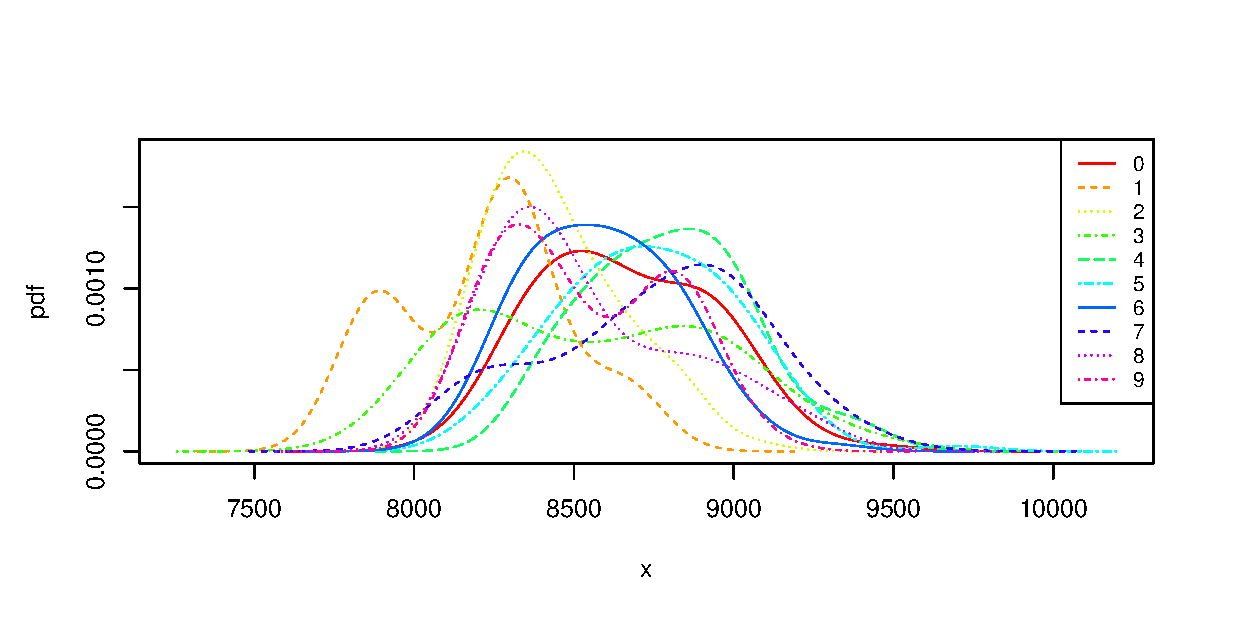
\includegraphics[width = \textwidth]{graphics/kde_graphs_sum}
    \caption{Density plot for each classification. The sum of all pixels are compared.}
    \label{fig:pdf_sum_kde}
\end{figure}

To see if it was possible to differentiate the data without increasing the dimensions, different summation techniques were tried. 
In figure \ref{fig:pdf_gaussian_kde} a Gaussian sum was compared. Weighting the data closest to the center higher than the data far away gave a different result although the data still overlaps.
In table \ref{tb:kde_confus} the classifications is displayed. 
If a better way to differentiate the data is used it could be useful to test as the data it was able to detect had above 48\% successful detections.

\begin{figure}[H]
    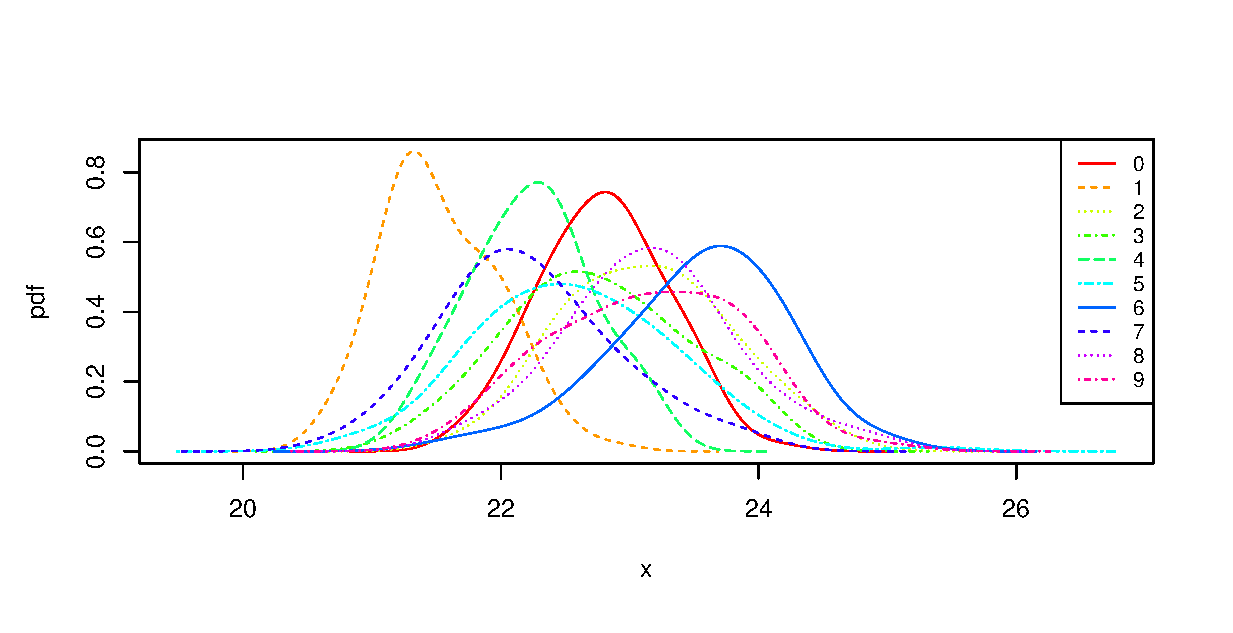
\includegraphics[width = \textwidth]{graphics/kde_graphs}
    \caption{Density plot for each classification. A Gaussian sum was compared.}
    \label{fig:pdf_gaussian_kde}
\end{figure}

\begin{table}[H]
\centering
         \begin{subtable}{0.75\textwidth}
        \centering
        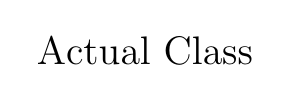
\begin{tikzpicture}
            \node at (0,0) {\Large Actual Class}; 
        \end{tikzpicture}
    \end{subtable}
    
    \begin{subtable}{0.05\textwidth}
        \flushright
        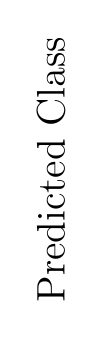
\begin{tikzpicture}
            \node[rotate=90] {\Large Predicted Class};
        \end{tikzpicture}
    \end{subtable}
    \begin{subtable}{0.7\textwidth}
            \centering
%            {\scriptsize
                \begin{tabular}{l|*{10}{c}}
                    &0	& 1	& 2	& 3	& 4	& 5	& 6	& 7	& 8	& 9 \\
\hline
0	& 0	& 0	& 0	& 0	& 0	& 0	& 0	& 0	& 0	& 0 \\
1	& 0	& 41	& 1	& 3	& 0	& 0	& 0	& 0	& 0	& 3 \\
2	& 26	& 53	& 19	& 13	& 25	& 28	& 18	& 5	& 7	& 30 \\
3	& 0	& 0	& 0	& 3	& 0	& 0	& 1	& 1	& 0	& 1 \\
4	& 34	& 2	& 41	& 37	& 41	& 31	& 39	& 51	& 49	& 23 \\
5	& 0	& 0	& 2	& 1	& 0	& 0	& 4	& 2	& 1	& 1 \\
6	& 31	& 4	& 29	& 18	& 11	& 19	& 19	& 4	& 14	& 22 \\
7	& 9	& 0	& 8	& 25	& 23	& 22	& 19	& 37	& 29	& 20 \\
8	& 0	& 0	& 0	& 0	& 0	& 0	& 0	& 0	& 0	& 0 \\
9	& 0	& 0	& 0	& 0	& 0	& 0	& 0	& 0	& 0	& 0 \\

                    \multicolumn{11}{l}{\bf Success}\\
                    \multicolumn{1}{l}{}&0.49&0.48&0.00&0.00&0.55&0.00&0.82&0.00&0.04&0.00\\
                \end{tabular}
%            }
    \end{subtable}
    \caption{Confusion matrix for KDE.}
    \label{tb:kde_confus}
\end{table}
